\documentclass[tizk]{standalone}

\usepackage{fontspec}
\setmainfont{LexendDeca}
\setsansfont{montserrat}
\setmonofont{Cascadia Code PL}

\usepackage[fixed]{fontawesome5}
\usepackage{tikz}
\usetikzlibrary{positioning}
\usetikzlibrary{arrows}
\usetikzlibrary{decorations}
\usetikzlibrary{shapes.symbols}

\begin{document}

\begin{tikzpicture}[
    scale=2,
    ->,>=latex,shorten >=1pt,
    node distance=.5cm,
    bend angle=15,
    every node/.append style={align=center},
    rectangle/.append style={draw,fill=white},
]
    \node[draw,shape=cloud,cloud puffs=20,cloud puff arc=120,aspect=6] (environment) {Environnement};
    \node[rectangle,above=of environment] (harware) {Matériel};
    \node[rectangle,above=of harware] (bootloader) {Bootloader};
    \node[rectangle,above=of bootloader] (kernel) {Noyau \& système};
    \node[rectangle,above=of kernel] (software) {Logiciel};
    \node[above=of software] (user) {\Large\faIcon{grin-beam}};
    
    \draw (environment) edge (harware);
    \draw (harware) edge (bootloader);
    \draw (bootloader) edge (kernel);
    \draw (kernel) edge (software);
    \draw (software) edge (user);
\end{tikzpicture}

\end{document}